\documentclass{article}
\def\ntitle {Orthogonalization via Polar Decomposition}
% \def\nauthor{ } % default author is Zhengbo Zhou
% \def\notes{ } % default is the submitted version
% \def\ndate{ } % default is today's date
% \def\needcrop{ } % crop for easy previewing
% \def\fancysec{ } % section font become fancier 
\RequirePackage{etex}
\makeatletter
\ifx \nauthor\undefined
  \def\nauthor{Zhengbo Zhou}
\else 
\fi 
\ifx \ndate\undefined 
  \def\ndate{\today}
\else 
\fi 

\author{\nauthor \thanks{%
Department of Mathematics,
University of Manchester,
Manchester, M13 9PL, England
(\texttt{zhengbo.zhou@postgrad.manchester.ac.uk}).
}}
\date{\ndate}
\title{\ntitle}

% RedeclareMathOperator
\newcommand\RedeclareMathOperator{%
  \@ifstar{\def\rmo@s{m}\rmo@redeclare}{\def\rmo@s{o}\rmo@redeclare}%
}
% this is taken from \renew@command
\newcommand\rmo@redeclare[2]{%
  \begingroup \escapechar\m@ne\xdef\@gtempa{{\string#1}}\endgroup
  \expandafter\@ifundefined\@gtempa
     {\@latex@error{\noexpand#1undefined}\@ehc}%
     \relax
  \expandafter\rmo@declmathop\rmo@s{#1}{#2}}
% This is just \@declmathop without \@ifdefinable
\newcommand\rmo@declmathop[3]{%
  \DeclareRobustCommand{#2}{\qopname\newmcodes@#1{#3}}%
}
\@onlypreamble\RedeclareMathOperator

\usepackage{algorithm}
\usepackage{algpseudocode}
\usepackage{comment}
\usepackage{bookmark}
\usepackage{microtype}
\usepackage{booktabs}
\usepackage{lastpage}
\usepackage{fancyhdr}
\usepackage{amsthm}
\usepackage{mathtools}
\usepackage{enumerate}
\usepackage{mathrsfs}
\usepackage{amsfonts}
\usepackage{amssymb}
\usepackage{tcolorbox}
\usepackage{bm}
\usepackage{cancel}
\usepackage{bbm}
\usepackage{accsupp}
\usepackage{enumitem}
\usepackage{hyperref}
\usepackage[fontsize=12pt]{fontsize}
\usepackage{geometry}
\usepackage{microtype}
\usepackage{algorithm,algorithmicx,algpseudocode}

\hbadness=99999

\geometry{
  a4paper,
  textwidth=165truemm,
  textheight=240truemm,
  top=28.5truemm,
}

\let\LaTeXStandardTableOfContents\tableofcontents
\renewcommand{\tableofcontents}{%
\begingroup%
\renewcommand{\bfseries}{\sc}%
\LaTeXStandardTableOfContents%
\endgroup%
}%
\setcounter{tocdepth}{3}
\makeatletter
\renewcommand\tableofcontents{\@starttoc{toc}}
\makeatother

\hypersetup{
  hypertexnames=false, 
  colorlinks=true,
  linkcolor=blue,
  pdfauthor={Zhengbo Zhou},
  pdftitle={\ntitle},
  pdfcreator={Zhengbo Zhou via MikTeX}
}

\usepackage[hyperpageref]{backref}
\renewcommand*{\backref}[1]{}
\renewcommand*{\backrefalt}[4]{
    \ifcase #1 %
    No citations.%
    \or
    (Cited on p.~#2.)
    \else
    (Cited on pp.~#2.)
    \fi
}



\pagestyle{fancyplain}
\fancyhead[R]{{\textit{\footnotesize\nouppercase Short Course : Function of Matrices}}}
\fancyhead[L]{\footnotesize\nouppercase\leftmark}


\newtcolorbox{mybox}[1]{colback=white!90!black,colframe=white!40!black,fonttitle=\scshape\centering,title=#1}

%%% MATLAB Code From Dr. Chris Johnson 
\usepackage{color}  
\usepackage{xcolor}
\usepackage{listings}
\definecolor{codegreen}{rgb}{0,0.6,0}
\definecolor{codegray}{rgb}{0.5,0.5,0.5}
\definecolor{codepurple}{rgb}{0.58,0,0.82}
\definecolor{mygreen}{RGB}{28,172,0}
\definecolor{mylilas}{RGB}{170,55,241}
\definecolor{backcolour}{rgb}{0.95,0.95,1.92}
\lstdefinestyle{mystyle}{
	language=matlab,
    commentstyle=\color{codegreen},
    keywordstyle=\color{blue},
    numberstyle=\footnotesize\color{codegray},
    stringstyle=\color{codepurple},
    basicstyle=\linespread{1}\ttfamily\small,
    breakatwhitespace=false,
    breaklines=true,
    captionpos=b,
    keepspaces=true,
    numbers=left,
    numbersep=10pt,
    showspaces=false,
    showstringspaces=false,
    showtabs=false,
    tabsize=4,
    aboveskip=\medskipamount,
    % frame=single,
}
\lstset{style=mystyle}
\def\inline{\lstinline[basicstyle=\upshape\ttfamily]}

%% Theorems 
\newtheorem{theorem}{Theorem}[section]
\newtheorem{proposition}[theorem]{Proposition}
\newtheorem{corollary}[theorem]{Corollary}
\newtheorem{lemma}[theorem]{Lemma}
\theoremstyle{definition}
\newtheorem{definition}[theorem]{Definition}
\newtheorem{example}[theorem]{Example}
\newtheorem{remark}[theorem]{Remark}
\newtheorem*{question}{Question}
\newtheorem*{recall}{Recall}
\newtheorem*{assumption}{Assumption}
\newtheorem*{note}{Note}
\numberwithin{equation}{section}

\let\stdsection\section
\renewcommand\section{\newpage\stdsection}

%%% Paired labels
\DeclarePairedDelimiter\ceil{\lceil}{\rceil}
\DeclarePairedDelimiter\floor{\lfloor}{\rfloor} 
\DeclarePairedDelimiter\abs{\lvert}{\rvert} % |a|
\DeclarePairedDelimiter\inner{\langle}{\rangle} % <a>
\makeatletter
\let\oldabs\abs
\def\abs{\@ifstar{\oldabs}{\oldabs*}}

%%%------------------------------------------------------------------%%%

%%% vector bold
\renewcommand{\vec}[1]{\bm{#1}}

%%%------------------------------------------------------------------%%%

%%% Real and Imaginary
\RedeclareMathOperator{\Im}{\mathrm{Im}}
\RedeclareMathOperator{\Re}{\mathrm{Re}}

%%% Integrate from ... to ...       
\newcommand{\intii}{\int_{-\infty}^{\infty}}

%%% Greek Letters
% NEVER define \l for \lambda due to Polish names in BibTeX
\renewcommand{\L}{\Lambda}
\newcommand{\vL}{\varLambda}
\newcommand{\g}{\gamma}
\newcommand{\G}{\Gamma}
\newcommand{\vG}{\varGamma}
\renewcommand{\o}{\omega}
\renewcommand{\O}{\Omega}
\newcommand{\vO}{\varOmega}
\newcommand{\s}{\sigma}
\renewcommand{\S}{\Sigma}
\newcommand{\vS}{\varSigma}
\newcommand{\eps}{\varepsilon}
\newcommand{\lap}{\varDelta}

%%% Matrix Related
\newcommand{\n}{^{n}}
\newcommand{\m}{^{m}}
\newcommand{\Rn}{\R^n}
\newcommand{\mn}{^{m\times n}}
\newcommand{\nn}{^{n\times n}}
\newcommand{\tp}{^{T}} 
\newcommand{\ctp}{^{*}}
\newcommand{\inv}{^{-1}}
\DeclareMathOperator{\diag}{diag}
\DeclareMathOperator{\rank}{rank}
\DeclareMathOperator{\tr}{trace}
\DeclareMathOperator{\range}{Range}

%%%------------------------------------------------------------------%%%

%% Norms
\newcommand{\iter}[1]{^{(#1)}} % iteration
\newcommand{\gnorm}[1]{\left\|{#1}\right\|} % general norm
\newcommand{\norm}[1]{\gnorm{#1}}
\newcommand{\tnorm}[1]{\gnorm{#1}_2} % 2-norm
\newcommand{\inorm}[1]{\gnorm{#1}_\infty} % infinity norm

%%% Over the expressions
\newcommand{\wh}{\widehat}
\newcommand{\wt}{\widetilde}
\newcommand{\wb}{\overline}

%%% Calculus
\DeclareMathOperator{\grad}{\nabla}
\renewcommand{\div}{\nabla\cdot}
\DeclareMathOperator{\curl}{\nabla\times}
\newcommand{\dd}{\mathrm{d}}
\newcommand{\pp}{\partial}
\def\eu{\mathrm{e}} % euler's constant
\def\im{\mathrm{i}} % imaginary unit

%%% Citation
\def\ycite[#1#2#3#4#5]#6{\cite[$\mit{#1#2#3#4}$#5]{#6}}

%%%------------------------------------------------------------------%%%

%%% MATHBB
\newcommand{\mb}[1]{\mathbb{#1}}
\newcommand{\N}{\mb{N}}
\newcommand{\Z}{\mb{Z}} 
\newcommand{\Q}{\mb{Q}}
\newcommand{\R}{\mb{R}} 
\newcommand{\C}{\mb{C}}
\newcommand{\F}{\mb{F}}
\renewcommand{\P}{\mb{P}} % Probability
\newcommand{\E}{\mb{E}} % Expectation
\newcommand{\V}{\mb{V}} % Variance

%%% MATHCAL and MATHSCR
\newcommand{\mc}[1]{\mathcal{#1}} % For spaces 
\newcommand{\ms}[1]{\mathscr{#1}} % For sigma-algebra
\newcommand{\mf}[1]{\mathfrak{#1}}

%%%------------------------------------------------------------------%%%

%%% Stochastic Calculus
\newcommand{\ps}{$(\Omega,\ms F,\P)$}
\newcommand{\ito}{It\^o}
\DeclareMathVersion{bold}
\newcommand{\indi}{\mathbbm{1}} % indicator function
\providecommand*{\napprox}{%
  \BeginAccSupp{method=hex,unicode,ActualText=2249}%
  \not\approx
  \EndAccSupp{}%
}
\mathchardef\gang="2D
\DeclareMathOperator*{\esssup}{esssup}

\DeclareMathOperator{\law}{\mathfrak{Law}}
\newcommand{\loc}{\textup{loc}}
\newcommand{\locmart}{\mc M_{\loc}^C}
\newcommand{\locm}{\mc M_{\loc,T}^{C,0}}
\newcommand{\locmt}{\wt{\mc M}_{\loc,T}^{C,0}}
\newcommand{\nicee}[1]{\mathcal{E}_{#1}^H(B)}


\DeclareMathOperator{\sign}{diag}

\makeatother

%% redefine \emph and \bf such that they are colored and can be easily
%% transformed back to normal \emph and \bf
\renewcommand{\emph}[1]{\textit{\color{purple} #1}}
\renewcommand{\bf}[1]{\textsf{\bfseries \color{purple} #1}}

\numberwithin{equation}{section} % equation numbers

\begin{document}
\maketitle
% \tableofcontents
\thispagestyle{firstpage}
%%%%%%%%%%%%%%%%%%%%%%%%%%%%%%%%%%%%%%%%%%%%%%%%%%%%%%%%%%%%%%%%%%%%%%
%%%%%%%%%%%%%%%%%%%%%%%%%%%% MAIN ARTICLE %%%%%%%%%%%%%%%%%%%%%%%%%%%%
%%%%%%%%%%%%%%%%%%%%%%%%%%%%%%%%%%%%%%%%%%%%%%%%%%%%%%%%%%%%%%%%%%%%%%
% \begin{abstract}
% This note provide an alternative way for the orthogonalization process in
% mixed-precision Jacobi eigenvalue algorithm~\ycite[2022]{zhba22}.
% The matrix we get from the low precision eigendecomposition is an almost
% orthogonal matrix in high precision. The previous method uses the Modified
% Gram–Schmidt QR which does not utilize the fact that the input matrix $Q$ is
% almost orthogonal in the sense that $\norm{Q\tp Q - I} \lesssim 
% nu_{\mathrm{low}}$, where $u_{\mathrm{low}}$ is the unit roundoff of the
% low precision. 
% \end{abstract}

\section{Introduction}

\subsection{Preliminaries}
The norm, throughout this report, will be unitarily invariant norm.
Namely, for any $A\in\C\nn$, $\norm{QAP} = \norm{A}$ for any two unitary
matrices $Q,P \in \C\nn$.
One important property of the unitarily invariant norm is that
they are self-adjoint \ycite[2013, pp.~357-358]{hojo13_ma}, i.e.
$\norm{A\ctp} = \norm{A}$. This can be proved by considering the SVD
(Theorem~\ref{thm.svd}) of $A$. 

We will consider two precisions: high precision,
$u_{\mathrm{high}}$, and low precision, $u_{\mathrm{low}}$, such that
$u_{\mathrm{low}} \gg u_{\mathrm{high}}$.
For example, they can be interpreted as single precision (low) and double
precision (high), where 
$u_{\mathrm{single}} \approx 6 \times 10^{-8}$ and $u_{\mathrm{high}}
\approx 1.1 \times 10^{-16}$ by IEEE standard~\ycite[2019]{ieee19}.
The error analysis for the eigendecomposition in arbitrary precision is
readily presented by \cite[Sec.~4.7.1]{abbb99_lug}.
\begin{theorem}
\label{thm.lug-eig-error}
Let $A\in\R\nn$ be a symmetric matrix. The computed eigendecomposition $A =
\wt Z \wt \Lambda \wt Z\tp$ via any LAPACK routine in precision $u$ is
nearly the exact eigendecomposition of $A+E$.
Namely, $A + E = (\wt Z + \delta \wt Z)\wt \Lambda (\wt Z + \delta
\wt Z)\tp$ is a true eigendecomposition so that $\wt Z + \delta \wt Z$ is
orthogonal, where $\norm{E}/\norm{A} \le p(n)u$ and $\norm{\delta \wt Z}
\le p(n)u$. Here $p(n)$ is a modestly growing function of $n$.
\end{theorem}

\subsection{Orthogonalization via QR}
\label{sec.orth-via-qr}

In 2022, Zhang and Bai~\ycite[2022]{zhba22} propose a mixed precision Jacobi
algorithm that can be described by Algorithm~\ref{alg.mpja-zhangbai}.
%Algorithm Env
% You may use \For \EndFor \If \Else \ElsIf \EndIf
\begin{algorithm}
\caption{A summary of the mixed precision Jacobi algorithm for symmetric
  eigenvalue problem proposed by Zhang and Bai~\ycite[2022, Alg.~4.1]{zhba22}.} 
\label{alg.mpja-zhangbai}
\begin{algorithmic}[1]
\Require {A symmetric matrix $A\in\R\nn$.}
\Ensure {An orthogonal matrix $P \in \R\nn$ and a diagonal matrix $\Delta$.}
\State{Compute the eigendecomposition of $A$ in low precision, $A =
  P_{\mathrm{low}}\Delta_{\mathrm{low}}P_{\mathrm{low}}\tp$.}
\State{Compute an QR factorization of $P_{\mathrm{low}} = Q_{P}R_{P}$.}
\Comment{Modified Gram-Schmidt}
\State{Precondition the matrix $A$ by $A_{\mathrm{cond}} = Q_{P}\tp AQ_{P}$.}
\State{Apply Jacobi algorithm on $A_{\mathrm{cond}}$.}
\end{algorithmic}
\end{algorithm}

From the second step, the paper orthogonalizes the almost orthogonal
matrix $P_{\mathrm{low}}$ using the modified Gram-Schmidt QR factorization.
This method can compute the QR factors with a small residual.
Moreover, the computed orthogonal factor $Q_{P}$ has a bounded departure from
orthonormality, i.e. $\tnorm{Q_{P}\tp Q_{P} - I}$ is bounded by some multiple
of $u_{\mathrm{high}}\kappa_{2}(P_{\mathrm{low}})$~\ycite[2013,
Sec.~5.2.9]{gova13_mc4}.   
The cost of the modified Gram-Schmidt algorithm is $2n^{3}$ for $n\times n$
matrix~\ycite[2013, Alg.~5.2.6]{gova13_mc4}.
Moreover, the input matrix for the MGS algorithm, $P_{\mathrm{low}}$, is a
computed eigenvector matrix in precision $u_{\mathrm{low}}$. Notice that,
although the MGS QR decomposition may produce a large deviation from
orthogonality, but due to the excellent condition of $P_{\mathrm{low}}$,
the bound will be roughly a multiple of $u_{\mathrm{high}}$.

\begin{theorem}
\label{thm.bound-on-norm-Plow}
Let $P_{\mathrm{low}}$ be an computed eigenvector matrix via any LAPACK
routine in precision $u_{\mathrm{low}}$. Then, we have the upper bound for
the 2-norm of $P_{\mathrm{low}}$,
\begin{equation}\notag
  \tnorm{P_{\mathrm{low}}} \le 
  p(n)u_{\mathrm{low}} + \sqrt{1 + 2p(n)^{2}u_{\mathrm{low}}^{2}}
\end{equation}
where $p(n)$ is a modestly increasing function of $n$.
\end{theorem}

\begin{proof}
By Theorem~\ref{thm.lug-eig-error}, we have
\begin{equation}\notag
  (P_{\mathrm{low}} + \delta P_{\mathrm{low}}) \tp
  (P_{\mathrm{low}} + \delta P_{\mathrm{low}}) = I, \qquad
  \norm{\delta P_{\mathrm{low}}} \le p(n)u_{\mathrm{low}},
\end{equation}
where $p(n)$ is a modestly growing function in $n$.
Multiply out we have 
\begin{equation}\notag
  P_{\mathrm{low}}\tp P_{\mathrm{low}} + P_{\mathrm{low}}\tp
  \delta P_{\mathrm{low}} + \delta P_{\mathrm{low}} \tp 
  P_{\mathrm{low}} + \delta P_{\mathrm{low}} \tp \delta P_{\mathrm{low}}
  = I.
\end{equation}
Let us concentrate on the 2-norm and substitute $\norm{\delta P_{\mathrm{low}}}
\le p(n)u_{\mathrm{low}}$,
\begin{equation}\notag
  \tnorm{P_{\mathrm{low}}}^{2} \le \tnorm{I} + 2 p(n)u_{\mathrm{low}}
  \tnorm{P_{\mathrm{low}}} + p(n)^{2} 
  u_{\mathrm{low}}^{2},
\end{equation}
and the solution to this inequality is
\begin{equation}\label{eq.bound-on-normA}
  \tnorm{P_{\mathrm{low}}} \le 
  p(n)u_{\mathrm{low}} + \sqrt{1 + 2p(n)^{2}u_{\mathrm{low}}^{2}},
\end{equation}
which proves the claim.
\end{proof}

This theorem will be useful when we consider the convergence of the
Newton--Schulz iteration for computing the unitary polar factor of
$P_{\mathrm{low}}$ as the Newton--Schulz iteration, unlike the Newton iteration,
in Section~\ref{sec.newt-schulz-iter},
Theorem~\ref{thm.conv-newton-schulz}, is only locally convergent.

\section{Polar Decomposition}
Before introducing the polar decomposition, the singular value decomposition
(SVD) for a squared matrix is necessary to be described here.
\begin{theorem}[singular value decomposition]
\label{thm.svd}
Let $A\in\C\nn$, there exist unitary matrices $U,V \in \C\nn$ such that
\begin{equation}\notag
  U\ctp A V = \Sigma = \diag(\sigma_{1},\dots,\sigma_{n}) \in \R\nn,
\end{equation}
where $\sigma_{1} \ge \sigma_{2} \ge \cdots \ge \sigma_{n} \ge 0$.
We will denote the decomposition $A = U\Sigma V\ctp$ as the singular value
decomposition (SVD) of $A$, and the diagonal entries of $A$ are called the
singular values of $A$.
\end{theorem}

The polar decomposition can be then defined with the help of the SVD.
\begin{theorem}[polar decomposition]
Let $A\in\C\nn$ have full rank.
There exists a unique unitary matrix $U_{A}\in\C\nn$
and a unique Hermitian positive definite matrix $H_{A}\in\C\nn$
such that $A = U_{A}H_{A}$. The uniqueness of $H_{A}$ comes from
\begin{equation}\notag
  (A\ctp A)^{1/2} = (H_{A}\ctp U_{A}\ctp U_{A}H_{A})^{1/2} =
  (H_{A}^{2})^{1/2} = H_{A}, 
\end{equation}
and every Hermitian positive definite matrix has a unique Hermitian positive
definite square root~\ycite[2008, Cor.~1.30]{high08_fm}. $U_{A} = A H_{A}\inv$
will ensure the uniqueness of $U_{A}$.
\end{theorem}
This can be proved by using SVD. Let $A\in\C\nn$ have full rank with
SVD $A = U\Sigma V\ctp$, then $\sigma_{i} > 0$ for all $i = 1:n$.
Then we can rewrite the SVD in the following form
\begin{equation}\notag
  A = U\Sigma V\ctp = (UV\ctp) (V\Sigma V\ctp) \coloneqq U_{A} H_{A}.
\end{equation}
With this definition of $U_{A}$ and $H_{A}$, all the conditions in the
previous 
theorem can be easily checked. We will refer to $U_{A}$ as the unitary polar
factor and $H_{A}$ as the Hermitian polar factor. 

It is sufficient to only consider the square, nonsingular matrices for the polar
decomposition. Let $A\in\C\mn$ with $m\geq n$ have 
the QR factorization $A = QR$ where $Q\in\C^{m\times n}$ and $R\in\C\nn$.
Then find the polar decomposition $R = UH$ and $A = QU\cdot H$ becomes the
polar decomposition of $A$. In addition, if $A\in\C\mn$ is singular, we can
compute a complete orthogonal decomposition
\begin{equation}\notag
  A = P
  \begin{bmatrix}
    R & 0 \\ 0 & 0 
  \end{bmatrix}
  Q\ctp,
\end{equation}
where $P,Q$ are unitary, and $R\in\C^{r\times r}$ is nonsingular and upper
triangular. % For more details of this decomposition, you may refer to
% Bj\"{o}rck~\ycite[1996, Def.~1.3.1]{bjor96_nmflsp}.
Then, we may compute
the polar decomposition of $R$ and assemble them together by 
\ycite[1990, Sec.~2]{hisc90}.
The unitary polar factor of $A$ satisfies the best approximation
property~\ycite[2008, Sec. 8.1]{high08_fm}.
\begin{theorem}[best approximation]
\label{thm.best-approximation}
Let $A\in\C\nn$ have the polar decomposition $A = UH$.
Then $\norm{A - U} = \min \{ \norm{A-Q} : Q\ctp Q = I\}$ for any unitarily
invariant norm. 
\end{theorem}

Due to the best approximation property, considering the matrix
$P_{\mathrm{low}}$ in Algorithm~\ref{alg.mpja-zhangbai}, the polar
decomposition  will give the unitary matrix that is closest to the input
matrix.
Moreover, the key benefit of using the polar decomposition over the QR
decomposition is that the unitary polar factor can be computed via
iteration with matrix multiplication only.

\section{Computing the Unitary Polar Factor}
\label{sec.comp-polar-decomp}

A straightforward way of computing the unitary polar factor is using SVD.
% You may use \For \EndFor \If \Else \ElsIf \EndIf \Comment
% \Require and \Ensure
\begin{algorithm}
\caption{Compute the unitary polar factor of $A\in\R\nn$ using the SVD.}
\label{alg.polar-svd}
\begin{algorithmic}[1]
\State{Compute the SVD of $A$, $A = U\Sigma V\ctp$.}
\State{Compute the unitary polar factor via $U_{A} = UV\ctp$.}
\end{algorithmic}
\end{algorithm}

However, due to not exploiting the almost orthogonal structure, this
algorithm is not competitive with the QR factorization, since the typical
cost of computing the full SVD is about $26n^{3}$ \ycite[2013,
Fig.~8.6.1]{gova13_mc4}. A more practical iterative method will be provided
in the next section.

\subsection{Newton Method}
The Newton iteration for the unitary polar factor can be deduced by apply
the Newton method to the equation $X\ctp X = I$.
Let $Y$ be an approximate solution, and then define the correction term
$E = X - Y$. Substitute $X = Y + E$ into $X\ctp X = I$, we have
$Y\ctp Y + Y\ctp E + E\ctp Y + E\ctp E = I$.
Drop the second order term in $E$
gives the Newton iteration for the unitary polar factor
\begin{equation}
  \label{eq.sylv-newton}
  \begin{aligned}
    E_{k}\ctp Y_{k} + Y_{k}\ctp E_{k} & = I - Y_{k}\ctp Y_{k}. \\
    Y_{k+1} & = Y_{k} + E_{k},  \\
    k = 0,1,\dots, &\ \text{and $Y_{0}$ is given}.
  \end{aligned}
\end{equation}
This form of the Newton method requires a solution for the
Sylvester equation at each step, and the cost for solving the Sylvester
equation is $O(n^{3})$. Instead, we can point out one solution to the
Sylvester equation $E_{k} = (Y_{k} - Y_{k}^{-*})/2$, and substitute into
the Newton iteration \eqref{eq.sylv-newton}, we have the Newton iteration
\begin{equation}\label{eq.cls-newton}
  Y_{k+1} = \frac{1}{2}(Y_{k}^{-*} + Y_{k}), \qquad Y_{0} = A \in \C\nn,
  \text{ nonsingular}.
\end{equation}
Notice, we choose the starting point of our iteration to be $A$. This is
essential for the convergence result in \ycite[1986, Sec. 3.2]{high86p}. 

\subsection{Newton Schulz Iteration}
\label{sec.newt-schulz-iter}
The drawback of the Newton iteration is that it requires the explicit form
of an inverse of a matrix during each step.
To use the fact that the matrix multiplication is very fast on
high-performance computers, one can transform this inversion into two matrix
multiplications by using the Schulz iteration for matrix inverse.
Instead of computing the all the way until we got an inverse
at each step, we use the one-step Schulz iteration to approximate the
inverse of $Y_{k}\ctp$, namely
\begin{equation}\notag
  Y_{k}^{-*} \approx X_{0}(2I - Y_{k}\ctp X_{0}), \qquad
  \text{$X_{0}$ is given.}
\end{equation}
According to \ycite[1995]{beni65}, $X_{0}$ should be an approximation to
$Y_{k}\inv$.
Consider the situation we have in Algorithm~\ref{alg.mpja-zhangbai},  
$Y_{0} = P_{\mathrm{low}}$ is an almost orthogonal matrix.
Therefore, in case $Y_{k}$ converges to an unitary matrix, $Y_{k}$
should be an increasingly good approximation to $Y_{k}^{-*}$.
Hence, we can let $X_{0} = Y_{k}$ for each step, and obtain the
following coupled iteration 
\begin{equation}\notag
  \begin{aligned}
    Z_{k} & = Y_{k} (2I- Y_{k}\ctp Y_{k}),\\
    Y_{k+1} & = \frac{1}{2}(Z_{k} + Y_{k}),
              \qquad Y_{0} = A, \quad k = 0,1,\dots,
  \end{aligned}
\end{equation}
or more compactly, we have the Newton--Schulz iteration for the unitary
polar factor of $A$,
\begin{equation}\notag
  Y_{k+1} = \frac{1}{2}Y_{k}(3I - Y_{k}\ctp Y_{k}),\qquad X_{0} = A.
\end{equation}
Notice that, at each step, we require 2 matrix multiplication instead of an
inversion. The Newton--Schulz iteration, unfortunately, is only locally
convergent, and can be characterized by the following theorem.

\begin{theorem}[convergence of Newton--Schulz iteration]
\label{thm.conv-newton-schulz}
Let $A\in\C\nn$ have full rank with the polar decomposition $A = UH$ and
$\sigma_{i}(A) \in (0,\sqrt{3})$. Then the Newton--Schulz iteration
converges to the unitary polar factor $U$ quadratically, and
\begin{equation}\notag
  \tnorm{Y_{k+1} - U} \le \frac{1}{2}\tnorm{Y_{k} + 2U}\tnorm{Y_{k}-U}^{2}.
\end{equation}
Moreover, let $R_{k} = I - X_{k}\ctp X_{k}$, then the convergence can be
viewed as
\begin{equation}\notag
  R_{k+1} = \frac{3}{4} R_{k}^{2} + \frac{1}{4} R_{k}^{3}.
\end{equation}
\end{theorem}
\begin{proof}
See problem 8.20 in \ycite[2008]{high08_fm}.
\end{proof}

% algorithm, stopping criterion, SVD

Since the Newton--Schulz iteration is only locally convergent, the next corollary
provide a sufficient condition on $P_{\mathrm{low}}$ for the convergence of the
iteration.

\begin{corollary}
\label{col.conv-nsiter-condi}
Let $P_{\mathrm{low}}$ be a computed eigenvector matrix via any LAPACK routine
in precision $u_{\mathrm{low}}$ with $p(n)$ defined in
Theorem~\ref{thm.lug-eig-error}. If $p(n)u_{\mathrm{low}} \le \sqrt{5} -
\sqrt{3}$, then $\tnorm{P_{\mathrm{low}}} < \sqrt{3}$. Moreover, the
Newton--Schulz method will converge by Theorem~\ref{thm.conv-newton-schulz}. 
\end{corollary}
\begin{proof}
From Theorem~\ref{thm.bound-on-norm-Plow}, we have
\begin{equation}\notag
  \tnorm{P_{\mathrm{low}}} \le
  p(n)u_{\mathrm{low}} + \sqrt{1 + 2p(n)^{2}u_{\mathrm{low}}^{2}}.
\end{equation}
By Theorem~\ref{thm.conv-newton-schulz}, the Newton--Schulz iteration on
$P_{\mathrm{low}}$ converges to its unitary polar factor $U_{P}$ if
$\sigma_{i}(P_{\mathrm{low}}) \in (0,\sqrt{3})$. Since all the singular values
are positive, the condition is equivalent to $\tnorm{P_{\mathrm{low}}} =
\sigma_{1} < \sqrt{3}$. In order to bound the right-hand side by $\sqrt{3}$,
by solving quadratic equation, we have $p(n) u_{\mathrm{low}} < \sqrt{5}
- \sqrt{3}$. 
\end{proof}

Notice that this condition is easy to satisfy since $p(n) \approx n$ in  
practice.  
Suppose the low precision is single precision,
$u_{\mathrm{low}} \approx 6 \times 10^{-8}$, then as long as the size
of the matrix does not exceed about $10^{7}$, then we have guaranteed
convergence for the Newton--Schulz iteration based on
Corollary~\ref{col.conv-nsiter-condi}.
Therefore, from now on, we should assume that $p(n)u_{\mathrm{low}} \ll 1$.
Assemble them, we have the following algorithm
%Algorithm Env
% You may use \For \EndFor \If \Else \ElsIf \EndIf \Comment
% \Require and \Ensure
\begin{algorithm}
\caption{Newton--Schulz iteration on $P_{\mathrm{low}}$, an
  eigenvector matrix computed via any LAPACK routine in precision
  $u_{\mathrm{low}}$.
  The algorithm will orthogonalize $P_{\mathrm{low}}$
  to $P_{\mathrm{high}}$ such that
  $\norm{P_{\mathrm{high}}\ctp P_{\mathrm{high}}- I} \le nu_{\mathrm{high}}$
  where  $u_{\mathrm{high}} \ll u_{\mathrm{low}}$.} 
\label{alg.ns-iter-orthogonal}
\begin{algorithmic}[1]
\State{$X_{0} = P_{\mathrm{low}}$}
\For{$i = 0,1,2,\cdots$, until converge}
\State{Compute $X_{i}\ctp X_{i}$}
\Comment{1 matrix-matrix multiplication}
\If {$\norm{X_{i}\ctp X_{i} - I} \le nu_{\mathrm{high}}$}
\State{\textbf{Break}, $P_{\mathrm{high}} = X_{i}$, \textbf{Quit}.}
% \ElsIf
% \Else
\EndIf
\State{Compute $X_{i+1} = \frac{1}{2}(3X_{i} - X_{i}(X_{i}\ctp X_{i})).$}
\Comment{1 matrix-matrix multiplication}
\EndFor
\end{algorithmic}
\end{algorithm}

Algorithm~\ref{alg.ns-iter-orthogonal} is an iterative refinement on
$P_{\mathrm{low}}$, and it is hard to analyze its complexity. However, it
turns out that this algorithm can converge very fast.
To see this, we need an upper bound on $\tnorm{I - P_{\mathrm{low}}\tp
  P_{\mathrm{low}}}$. 

\begin{corollary}
\label{cor.bound-on-orthog}
Let $P_{\mathrm{low}}$ be an computed eigenvector matrix via any LAPACK
routine in precision $u_{\mathrm{low}}$. Then we have
\begin{equation}\notag
  \tnorm{I - P_{\mathrm{low}}\tp P_{\mathrm{low}}} \le
  2 p(n)u_{\mathrm{low}} + O(p(n)^{2}u_{\mathrm{low}}^{2}),
\end{equation}
where $p(n)$ is a modestly increasing function of $n$.
\end{corollary}
\begin{proof}
From Theorem~\ref{thm.lug-eig-error} and proof of
Theorem~\ref{thm.bound-on-norm-Plow}, we have
\begin{equation}\notag
  P_{\mathrm{low}}\tp P_{\mathrm{low}} + P_{\mathrm{low}}\tp
  \delta P_{\mathrm{low}} + \delta P_{\mathrm{low}} \tp 
  P_{\mathrm{low}} + \delta P_{\mathrm{low}} \tp \delta P_{\mathrm{low}} = I.
\end{equation}
where $\tnorm{\delta P_{\mathrm{low}}} \le p(n)u_{\mathrm{low}} =: \eps$,
and $p(n)$ is a modestly growing function of $n$.
Manipulate the above equation and taking any norm, we have
\begin{equation}\notag
  \tnorm{ I - P_{\mathrm{low}} \tp P_{\mathrm{low}} } \le
  2 \tnorm{\delta P_{\mathrm{low}}} \tnorm{P_{\mathrm{low}}} +
  \tnorm{\delta P_{\mathrm{low}}}^{2}.
\end{equation}
Using $\tnorm{\delta P_{\mathrm{low}}} \le \eps$, we have
\begin{equation}\notag
  \tnorm{I - P_{\mathrm{low}}\tp P_{\mathrm{low}}} \le
  2 \eps \tnorm{P_{\mathrm{low}}}  + \eps^{2}.
\end{equation}
Using Theorem~\ref{thm.bound-on-norm-Plow},
$\tnorm{P_{\mathrm{low}}} \le \eps + \sqrt{1 + 2\eps^{2}}$, we have 
\begin{equation}\notag
  \begin{aligned}
    \tnorm{I - P_{\mathrm{low}}\tp P_{\mathrm{low}}}
    & \le 2\eps (\eps + \sqrt{1 + 2\eps^{2}}) + \eps^{2} \\
    & \le 2\eps (\eps  + 1 + \sqrt{2}\eps) + \eps^{2}
      \qquad \sqrt{x + y} \le \sqrt{x} + \sqrt{y},\ \forall x, y \ge 0 \\
    & = 2 \eps + (3 + 2 \sqrt{2}) \eps^{2} = 2 \eps + O(\eps ^{2}). 
  \end{aligned}
\end{equation}
Substituting back, we have proved the claim.
\end{proof}

Using the matrix norm property \ycite[2013, Sec.~2.3.2]{gova13_mc4}, 
\begin{equation}\notag
  \fnorm{A}/\sqrt{n} \le \tnorm{A},\qquad A \in \R\nn.
\end{equation}
By Corollary~\ref{cor.bound-on-orthog}, we transform the matrix 2-norm to
Frobenius norm, and use the same definition $ p(n)u_{\mathrm{low}} =: \eps
\ll 1$, we have 
\begin{equation}\notag
  \fnorm{I - P_{\mathrm{low}}\tp P_{\mathrm{low}}} \le
  {2\sqrt{n}\eps} + O(\eps^{2}). 
\end{equation}
Let $P_{\mathrm{low}}$ have the SVD $U\Sigma_{P}V\ctp$, then using
the unitarily invariance and the definition of the Frobenius norm, we have 
\begin{equation}\notag
  \fnorm{I - P_{\mathrm{low}}\tp P_{\mathrm{low}}}^{2}
  = \fnorm{ I - \Sigma_{P}\tp \Sigma_{P}} = 
  (\sigma_{1}^{2} - 1)^{2} + \cdots +
  (\sigma_{n}^{2} - 1)^{2} \le
  2 \sqrt{n} \eps. 
\end{equation}
Since the terms in the summation are all positive, therefore
$(\sigma_{i}^{2} - 1)^{2} \le 2 \sqrt{n} \eps$ for $i = 1,\dots,n$.
This indicates that all the singular values of $P_{\mathrm{low}}$ are
wiggling about 1 and this explains the matrix $P_{\mathrm{low}}$ is
well conditioned.

Moreover, using Corollary~\ref{cor.bound-on-orthog} and
Theorem~\ref{thm.conv-newton-schulz}, we have, after one Newton--Schulz
iteration,  
\begin{align*}
  \tnorm{I - X_{1}\tp X_{1}}
  & \le \frac{3}{4}\tnorm{I - X_{0}\tp X_{0}}^{2} + 
    \frac{1}{4} \tnorm{I - X_{0}\tp X_{0}}^{3} \\
  & \le \frac{3}{4} (2\eps + O(\eps^{2}))^{2} +
    \frac{1}{4} (2\eps + O(\eps^{2}))^{3} \\
  & = 3 \eps^{2} + O(\eps^{3})
    = 3 p(n)^{2} u_{\mathrm{low}}^{2} +
    O(p(n)^{3} u_{\mathrm{low}}^{3}).
\end{align*}
If we require the iteration converged in one iteration, then we need
$3p(n)^{2}u_{\mathrm{low}}^{2} \le p(n)u_{\mathrm{high}}$, and this is 
equivalent to $u_{\mathrm{high}} \ge 3p(n)u_{\mathrm{low}}^{2}$.
Notice that we ignore the lower order term here,
since we are doing approximation here, and lower order term will not play
an significant role if $p(n)^{2}u_{\mathrm{low}}^{3} \ll 1$.
However, this condition is
not possible if we consider $u_{\mathrm{low}}$ and $u_{\mathrm{high}}$ as
single and double precision.
Therefore, we proceed to another iteration,
\begin{equation}\label{eq.devi-orth-2-steps}
  \tnorm{I - X_{2}\tp X_{2}}
  \le \frac{27}{4} \eps^{4} + O(\eps^{5})
  = \frac{27}{4} p(n)^{4} u_{\mathrm{low}}^{4} + O(p(n)^{5}
  u_{\mathrm{low}}^{5}). 
\end{equation}
Suppose we require the iteration converge in two iteration, then using the
same requirement, we have 
$6.75p(n)^{3}u_{\mathrm{low}}^{4} \le u_{\mathrm{high}}$.
Let us consider $u_{\mathrm{low}}$ and $u_{\mathrm{high}}$ as
single and double precision, and assume $p(n) = n$, then to achieve this
condition, we approximately need $n \le 10^{4}$.

%%%%%%%%%%%%%%%%%%%%%%%%%%%%%%%%%%%%%%%%%%%%%%%%%%%%%%%%%%%%%%%%%%%%%%
\subsection{Numerical Experiments}
\begin{example}\label{eg.qr-ns}
The first experiment using the almost orthogonal matrix, $P_{\mathrm{low}}$, 
generated by applying MATLAB builtin \texttt{eig()} at single precision to
symmetric matrix $A$ with geometrically distributed singular values.
The size of $A$ is varied from 10 to 3000 and generated by using MATLAB
command \texttt{round(linspace(10,3e3,1e2))}.
Although from previous analysis, it is no need to control the condition
number, but we set it as $\kappa(A) = 100$.
We will apply two different functions: (i) the 2 step Newton--Schulz
iteration; (ii) MATLAB builtin \texttt{qr}.
From \eqref{eq.devi-orth-2-steps}, using Newton--Schulz iteration, the
output $P_{\mathrm{high}}$ should satisfy $\tnorm{P_{\mathrm{high}}\tp
  P_{\mathrm{high}} - I} \le 6.75p(n)^{4}u_{\mathrm{low}}^{4}$. The
Householder QR decomposition (used by MATLAB \texttt{qr}) produces an
orthogonal matrix $Q$ that satisfies $\tnorm{Q\ctp Q - I} \le
q(n)u_{\mathrm{high}}$, where $q(n)$ is a modestly increasing function in
$n$. The choice of the dimension ensures Newton--Schulz iteration to
compute a more orthogonal result than the Householder QR factorization.
This can be seen from the experiment results. 

\begin{figure}[H]
\centering
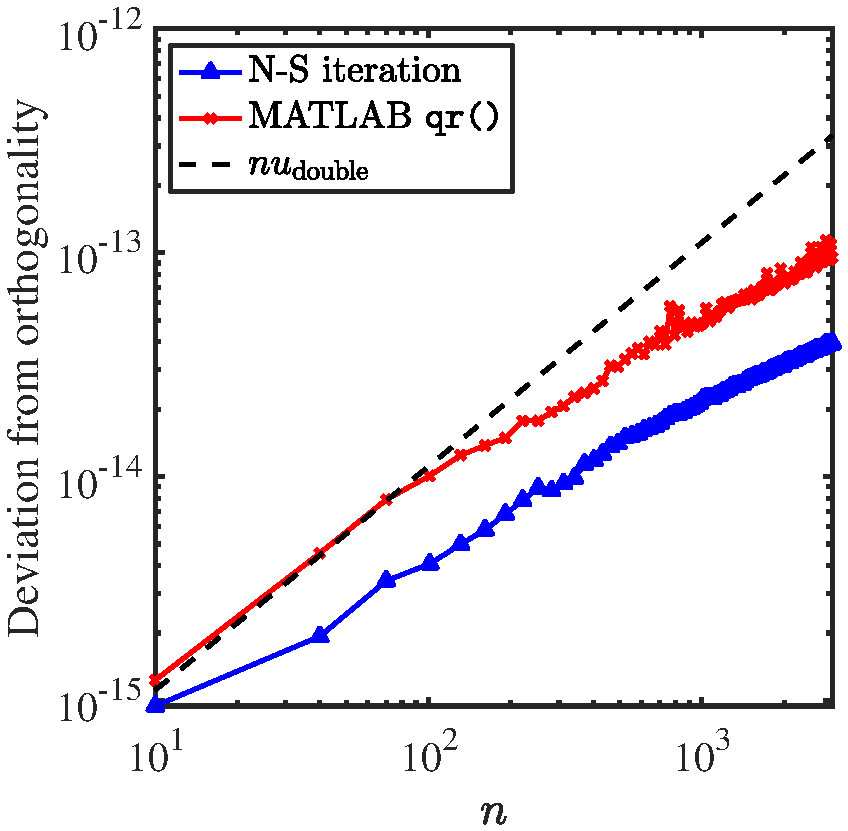
\includegraphics[width = 0.5 \textwidth]{./figs/ns-hqr.pdf}
\caption{Deviation from orthogonality after applying two Newton--Schulz
  iteration on the almost orthogonal matrix $P_{\mathrm{low}}$ described in
  Algorithm~\ref{alg.mpja-zhangbai}, compared with the MATLAB builtin
  \texttt{qr()}.} 
\label{fig.orthog-ns-qr}
\end{figure}

In Figure~\ref{fig.orthog-ns-qr}, we plot the deviation from orthogonality.
We see that after two iteration, the Newton--Schulz iteration will produce
a uniformly less deviation from orthogonality than the QR orthogonalization
process produced by \texttt{qr} function.
\end{example}

\begin{example}
Using the same setup as Example~\ref{eg.qr-ns}, we would like to further
compare the deviation from orthogonality between the 2 step Newton--Schulz
iteration and the modified Gram-Schmidt (MGS) QR factorization. The MATLAB
program for MGS is generate from the pseudo-code in \ycite[1998, Chap.~4,
Alg.~1.11]{stew98_ma}.

\begin{figure}[H]
\centering
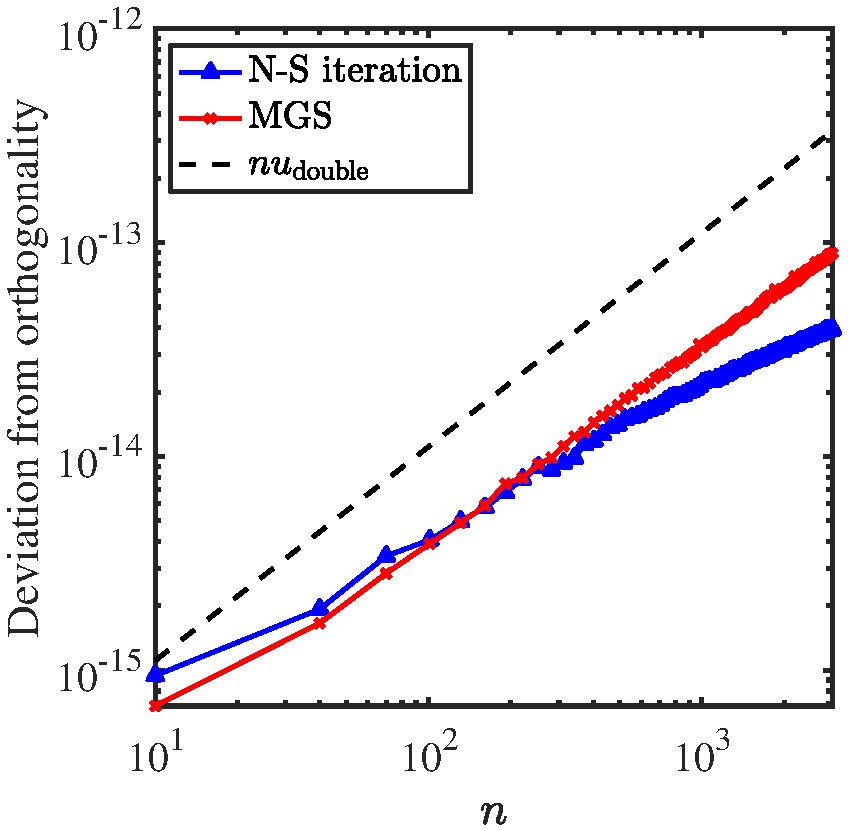
\includegraphics[width = 0.5 \textwidth]{./figs/ns-mgs.pdf}
\caption{Deviation from orthogonality after applying two Newton--Schulz
  iteration on the almost orthogonal matrix $P_{\mathrm{low}}$ described in
  Algorithm~\ref{alg.mpja-zhangbai}, compared with the MGS QR
  factorization.}  
\label{fig.orthog-ns-mgs}
\end{figure}

From Figure~\ref{fig.orthog-ns-mgs}, Newton--Schulz iteration is
competitive with the MGS, the suggested method by \ycite[2022]{zhba22}, in
terms of the orthogonality. These methods both produce an orthogonal matrix
in double precision. Although the gap between the trajectories is less
significant than the gap shown in Figure~\ref{fig.orthog-ns-qr}.
Newton--Schulz iteration produces an asymptotically smaller deviation from
orthogonality. 
\end{example}






%% Change the polynomial, the accuracy is not what we chosen, it is defined
%% by the method of eigendecomposition. In reality, most of the method will
%% have p(n) = n almost surely!
%% todo: change the previous things from sqrt(n) to n, shouldn't mentioned
%% n, since it is not mentioned in ASNA2 and zhba22!





%%%%%%%%%%%%%%%%%%%%%%%%%%%%%%%%%%%%%%%%%%%%%%%%%%%%%%%%%%%%%%%%%%%%%%
%%%%%%%%%%%%%%%%%%%%%%%%%%% Bibliographies %%%%%%%%%%%%%%%%%%%%%%%%%%%
%%%%%%%%%%%%%%%%%%%%%%%%%%%%%%%%%%%%%%%%%%%%%%%%%%%%%%%%%%%%%%%%%%%%%%
\newpage
\bibliographystyle{/Users/clement/Dropbox/bibtex/nj-plain}
\bibliography{/Users/clement/Dropbox/bibtex/strings.bib,
  /Users/clement/Dropbox/bibtex/misc.bib,
  /Users/clement/Dropbox/bibtex/ref.bib} 
\end{document}


%%% Local Variables:
%%% mode: latex
%%% TeX-master: t
%%% End:
